\begin{code}[hide]%
\>[0]\AgdaKeyword{module}\AgdaSpace{}%
\AgdaModule{slides.Tsinghua-PL-seminar.sections.newcore}\AgdaSpace{}%
\AgdaKeyword{where}\<%
\\
%
\\[\AgdaEmptyExtraSkip]%
\>[0]\AgdaKeyword{open}\AgdaSpace{}%
\AgdaKeyword{import}\AgdaSpace{}%
\AgdaModule{Data.Nat}\AgdaSpace{}%
\AgdaKeyword{using}\AgdaSpace{}%
\AgdaSymbol{(}\AgdaDatatype{ℕ}\AgdaSymbol{)}\<%
\\
\>[0]\AgdaKeyword{open}\AgdaSpace{}%
\AgdaKeyword{import}\AgdaSpace{}%
\AgdaModule{Data.Product}\AgdaSpace{}%
\AgdaKeyword{using}\AgdaSpace{}%
\AgdaSymbol{(}\AgdaRecord{Σ}\AgdaSpace{}%
\AgdaSymbol{;}\AgdaSpace{}%
\AgdaOperator{\AgdaFunction{\AgdaUnderscore{}×\AgdaUnderscore{}}}\AgdaSpace{}%
\AgdaSymbol{;}\AgdaSpace{}%
\AgdaOperator{\AgdaInductiveConstructor{\AgdaUnderscore{},\AgdaUnderscore{}}}\AgdaSymbol{)}\<%
\\
\>[0]\AgdaKeyword{open}\AgdaSpace{}%
\AgdaKeyword{import}\AgdaSpace{}%
\AgdaModule{Level}\AgdaSpace{}%
\AgdaKeyword{using}\AgdaSpace{}%
\AgdaSymbol{(}\AgdaFunction{0ℓ}\AgdaSymbol{)}\<%
\\
\>[0]\AgdaKeyword{open}\AgdaSpace{}%
\AgdaKeyword{import}\AgdaSpace{}%
\AgdaModule{Relation.Binary}\AgdaSpace{}%
\AgdaKeyword{using}\AgdaSpace{}%
\AgdaSymbol{(}\AgdaFunction{Rel}\AgdaSymbol{)}\<%
\\
\>[0]\AgdaKeyword{open}\AgdaSpace{}%
\AgdaKeyword{import}\AgdaSpace{}%
\AgdaModule{Relation.Nullary}\AgdaSpace{}%
\AgdaKeyword{using}\AgdaSpace{}%
\AgdaSymbol{(}\AgdaOperator{\AgdaFunction{¬\AgdaUnderscore{}}}\AgdaSymbol{)}\<%
\\
\>[0]\AgdaKeyword{open}\AgdaSpace{}%
\AgdaKeyword{import}\AgdaSpace{}%
\AgdaModule{Relation.Binary.PropositionalEquality}\AgdaSpace{}%
\AgdaKeyword{using}\AgdaSpace{}%
\AgdaSymbol{(}\AgdaOperator{\AgdaFunction{\AgdaUnderscore{}≢\AgdaUnderscore{}}}\AgdaSymbol{)}\<%
\\
\>[0]\AgdaKeyword{open}\AgdaSpace{}%
\AgdaKeyword{import}\AgdaSpace{}%
\AgdaModule{Algebra.Bundles}\AgdaSpace{}%
\AgdaKeyword{using}\AgdaSpace{}%
\AgdaSymbol{(}\AgdaRecord{Monoid}\AgdaSymbol{)}\<%
\\
%
\\[\AgdaEmptyExtraSkip]%
\>[0]\AgdaKeyword{open}\AgdaSpace{}%
\AgdaKeyword{import}\AgdaSpace{}%
\AgdaModule{Notations}\AgdaSpace{}%
\AgdaKeyword{using}\AgdaSpace{}%
\AgdaSymbol{(}\AgdaInductiveConstructor{₁₊}\AgdaSpace{}%
\AgdaSymbol{;}\AgdaSpace{}%
\AgdaInductiveConstructor{₂₊}\AgdaSymbol{)}\<%
\\
\>[0]\AgdaKeyword{open}\AgdaSpace{}%
\AgdaKeyword{import}\AgdaSpace{}%
\AgdaModule{Word.Base}\AgdaSpace{}%
\AgdaKeyword{using}\AgdaSpace{}%
\AgdaSymbol{(}\AgdaDatatype{Word}\AgdaSpace{}%
\AgdaSymbol{;}\AgdaSpace{}%
\AgdaFunction{WRel}\AgdaSpace{}%
\AgdaSymbol{;}\AgdaSpace{}%
\AgdaOperator{\AgdaInductiveConstructor{[\AgdaUnderscore{}]ʷ}}\AgdaSpace{}%
\AgdaSymbol{;}\AgdaSpace{}%
\AgdaInductiveConstructor{ε}\AgdaSpace{}%
\AgdaSymbol{;}\AgdaSpace{}%
\AgdaOperator{\AgdaInductiveConstructor{\AgdaUnderscore{}•\AgdaUnderscore{}}}\AgdaSpace{}%
\AgdaSymbol{;}\AgdaSpace{}%
\AgdaFunction{wmap}\AgdaSymbol{)}\<%
\\
%
\\[\AgdaEmptyExtraSkip]%
\>[0]\AgdaKeyword{postulate}\<%
\\
\>[0][@{}l@{\AgdaIndent{0}}]%
\>[2]\AgdaPostulate{proof-elided}\AgdaSpace{}%
\AgdaSymbol{:}\AgdaSpace{}%
\AgdaSymbol{∀}\AgdaSpace{}%
\AgdaSymbol{\{}\AgdaBound{ℓ}\AgdaSymbol{\}}\AgdaSpace{}%
\AgdaSymbol{\{}\AgdaBound{A}\AgdaSpace{}%
\AgdaSymbol{:}\AgdaSpace{}%
\AgdaPrimitive{Set}\AgdaSpace{}%
\AgdaBound{ℓ}\AgdaSymbol{\}}\AgdaSpace{}%
\AgdaSymbol{→}\AgdaSpace{}%
\AgdaBound{A}\<%
\\
%
\>[2]\AgdaPostulate{Gate}\AgdaSpace{}%
\AgdaSymbol{:}\AgdaSpace{}%
\AgdaDatatype{ℕ}\AgdaSpace{}%
\AgdaSymbol{→}\AgdaSpace{}%
\AgdaPrimitive{Set}\<%
\\
%
\>[2]\AgdaPostulate{X}\AgdaSpace{}%
\AgdaSymbol{:}\AgdaSpace{}%
\AgdaPrimitive{Set}\<%
\\
%
\\[\AgdaEmptyExtraSkip]%
\>[0]\AgdaKeyword{private}\AgdaSpace{}%
\AgdaKeyword{variable}\<%
\\
\>[0][@{}l@{\AgdaIndent{0}}]%
\>[2]\AgdaGeneralizable{n}\AgdaSpace{}%
\AgdaSymbol{:}\AgdaSpace{}%
\AgdaDatatype{ℕ}\<%
\end{code}
%% Part 6a — what happened after the submission; the core library.
\NewPart
\section{New since the paper}

\begin{frame}{What happened after the submission \New}
\begin{columns}[c]
\begin{column}{0.58\textwidth}
\centering
\begin{tikzpicture}[x=5.3mm,y=6.6mm,>={Stealth[length=1.6mm]},
  lb/.style={font=\scriptsize,anchor=west,align=left}]
  % trunk
  \draw[thick,paperC] (0,0) -- (3,0);
  \node[cm=paperC,label={[font=\scriptsize,align=center]below:tag\\[-2pt]\texttt{popl-revision1}}] at (0,0) {};
  \node[font=\tiny,gray] at (0,0.45) {Jul};
  \draw[thick,accent] (3,0) -- (6,0);
  \node[cm=accent,label={[font=\scriptsize]below:\texttt{main}}] at (6,0) {};
  \node[font=\tiny,gray] at (6,0.45) {Sep 2};
  % branches
  \draw[thick,newC] (6,0) .. controls (7,0) and (7,2.4) .. (9.5,2.4) node[cm=newC] {} node[lb,right=2pt]{\texttt{popl}\\[-1pt]path sums};
  \draw[thick,newC] (6,0) .. controls (7,0) and (7,0.8) .. (9.5,0.8) node[cm=newC] {} node[lb,right=2pt]{\texttt{v-office}\\[-1pt]unitary groups};
  \draw[thick,newC] (6,0) .. controls (7,0) and (7,-0.8) .. (9.5,-0.8) node[cm=newC] {} node[lb,right=2pt]{\texttt{qupit}\\[-1pt]minimality, CNOT-dihedral};
  \draw[thick,newC] (6,0) .. controls (7,0) and (7,-2.4) .. (9.5,-2.4) node[cm=newC] {} node[lb,right=2pt]{\texttt{v-office-Cli-CH}\\[-1pt]Real-Clifford+$CH$};
  \node[font=\scriptsize,align=center,accent] at (4.5,-1.6) {qupit Clifford,\\$Sp(2n,\mathbb{Z}_p)$,\\exact Clifford};
  \draw[->,gray] (4.5,-1.0) -- (4.5,-0.15);
  \node[font=\tiny,gray] at (9.5,3.1) {late Sep -- Oct 2026};
\end{tikzpicture}
\end{column}
\begin{column}{0.40\textwidth}
\centering
\begin{tikzpicture}
\begin{axis}[xbar, width=5.4cm, height=5.2cm, xmin=0, xmax=230,
  symbolic y coords={v-office-Cli-CH,qupit,v-office,popl,main,tag},
  ytick=data, y tick label style={font=\scriptsize\ttfamily},
  x tick label style={font=\scriptsize}, xlabel={\scriptsize thousand lines of Agda},
  nodes near coords, nodes near coords style={font=\tiny},
  bar width=7pt, enlarge y limits=0.12, axis lines*=left]
\addplot[fill=paperC!70,draw=paperC] coordinates {(22.2,tag)};
\addplot[fill=newC!60,draw=newC] coordinates
  {(112.8,main) (193.9,popl) (155.2,v-office) (139.9,qupit) (187.1,v-office-Cli-CH)};
\end{axis}
\end{tikzpicture}

{\scriptsize \texttt{*.agda} outside \texttt{paper/}; 74 files at the tag,
634 on \texttt{v-office-Cli-CH}}
\end{column}
\end{columns}
\end{frame}

\begin{frame}{Research papers formalized since the submission \New}
\centering\scriptsize
\renewcommand{\arraystretch}{1.18}
\begin{tabular}{@{}p{4.0cm}p{2.7cm}p{2.6cm}p{4.0cm}@{}}
\toprule
paper formalized & gate set / group & semantics & status\\
\midrule
Bian, Li, Ross, van de Wetering, Zhao (QPL'26): qupit Clifford, all odd primes
  & $H,S,CZ$; $\text{Pauli}\rtimes Sp(2n,\mathbb{Z}_p)$ & symplectic maps, Pauli action & \textbf{complete}, every $n$, every odd prime $p$\\
Selinger (LMCS 2015): $n$-qubit Clifford & $\omega,H,S,CZ$ & $Sp(2n,2)$ + phases & \textbf{complete} (modulo scalars; scalars as extension)\\
Bian--Selinger (QPL'21): $U_n(\mathbb{Z}[\frac12,i])$ & two-level $X,K,i$ & \alert{matrices} over $\mathbb{Z}[\frac12,i]$ & \textbf{complete}, every $n$\\
Greylyn (2014); Bian--Selinger (QPL'22): 2-qubit Clifford+$T$ & $\omega,H_i,S_i,T_i,CZ$ & \alert{matrices} over $\mathbb{Z}[\frac1{\sqrt2},i]$ & \textbf{complete} ($n\le4$; faithful into $U_4$)\\
Bian--Selinger (QPL'23): 3-qubit Clifford+$CS$ & $S_i, CS, K_i, i$ & matrices over $\mathbb{Z}[\frac12,i]$ & in progress (steps 1 and 4 of the R--S chain)\\
Clément (2026): Real-Clifford+$CH$ & $H,Z,CZ,CH$ & \alert{matrices} over $\mathbb{Z}[\sqrt2]$ & sound; complete on $\le1$ qubit; $\ge2$ modulo Thm 4.4 (imported by the paper too) + Lemma 8.8 at 3--4 qubits\\
Amy--Chen--Ross (QPL'17): CNOT-dihedral & $\omega,X,T,CNOT$ & phase polynomials & sound; complete on 1 qubit; $n$ modulo imported lemmas\\
Amy (QPL'18): path sums & $H,S,CZ$ / $H,CNOT,R_k$ & exact sums over $\mathbb{Z}[\zeta]$ & Clifford equivalence in \alert{polynomial cost}\\
\bottomrule
\end{tabular}

\vspace{4pt}
{\scriptsize plus, in the core: 0-ary gates (scalars), independence of axioms, central and
factor-set extensions, generic circuit coset towers}
\end{frame}

\begin{frame}{Scalars: 0-ary gates, and a rule that became a theorem \New}
\begin{columns}[c]
\begin{column}{0.55\textwidth}
\small Global phases ($\omega$, $\zeta$, \ldots) live on no wire, at every width:
\begin{code}%
\>[0]\AgdaKeyword{data}\AgdaSpace{}%
\AgdaDatatype{Gen}\AgdaSpace{}%
\AgdaSymbol{:}\AgdaSpace{}%
\AgdaDatatype{ℕ}\AgdaSpace{}%
\AgdaSymbol{→}\AgdaSpace{}%
\AgdaPrimitive{Set}\AgdaSpace{}%
\AgdaKeyword{where}\<%
\\
\>[0][@{}l@{\AgdaIndent{0}}]%
\>[2]\AgdaInductiveConstructor{gate₀}\AgdaSpace{}%
\AgdaSymbol{:}\AgdaSpace{}%
\AgdaPostulate{Gate}\AgdaSpace{}%
\AgdaNumber{0}\AgdaSpace{}%
\AgdaSymbol{→}\AgdaSpace{}%
\AgdaDatatype{Gen}\AgdaSpace{}%
\AgdaGeneralizable{n}\<%
\\
%
\>[2]\AgdaInductiveConstructor{gate₁}\AgdaSpace{}%
\AgdaSymbol{:}\AgdaSpace{}%
\AgdaPostulate{Gate}\AgdaSpace{}%
\AgdaNumber{1}\AgdaSpace{}%
\AgdaSymbol{→}\AgdaSpace{}%
\AgdaDatatype{Gen}\AgdaSpace{}%
\AgdaSymbol{(}\AgdaInductiveConstructor{₁₊}\AgdaSpace{}%
\AgdaGeneralizable{n}\AgdaSymbol{)}\<%
\\
%
\>[2]\AgdaInductiveConstructor{gate₂}\AgdaSpace{}%
\AgdaSymbol{:}\AgdaSpace{}%
\AgdaPostulate{Gate}\AgdaSpace{}%
\AgdaNumber{2}\AgdaSpace{}%
\AgdaSymbol{→}\AgdaSpace{}%
\AgdaDatatype{Gen}\AgdaSpace{}%
\AgdaSymbol{(}\AgdaInductiveConstructor{₂₊}\AgdaSpace{}%
\AgdaGeneralizable{n}\AgdaSymbol{)}\<%
\\
%
\>[2]\AgdaOperator{\AgdaInductiveConstructor{\AgdaUnderscore{}↥}}%
\>[7]\AgdaSymbol{:}\AgdaSpace{}%
\AgdaDatatype{Gen}\AgdaSpace{}%
\AgdaGeneralizable{n}\AgdaSpace{}%
\AgdaSymbol{→}\AgdaSpace{}%
\AgdaDatatype{Gen}\AgdaSpace{}%
\AgdaSymbol{(}\AgdaInductiveConstructor{₁₊}\AgdaSpace{}%
\AgdaGeneralizable{n}\AgdaSymbol{)}\<%
\end{code}
\begin{code}[hide]%
\>[0]\AgdaFunction{Circuit}\AgdaSpace{}%
\AgdaSymbol{:}\AgdaSpace{}%
\AgdaDatatype{ℕ}\AgdaSpace{}%
\AgdaSymbol{→}\AgdaSpace{}%
\AgdaPrimitive{Set}\<%
\\
\>[0]\AgdaFunction{Circuit}\AgdaSpace{}%
\AgdaBound{n}\AgdaSpace{}%
\AgdaSymbol{=}\AgdaSpace{}%
\AgdaDatatype{Word}\AgdaSpace{}%
\AgdaSymbol{(}\AgdaDatatype{Gen}\AgdaSpace{}%
\AgdaBound{n}\AgdaSymbol{)}\<%
\\
\>[0]\AgdaFunction{CRel}\AgdaSpace{}%
\AgdaSymbol{:}\AgdaSpace{}%
\AgdaDatatype{ℕ}\AgdaSpace{}%
\AgdaSymbol{→}\AgdaSpace{}%
\AgdaPrimitive{Set₁}\<%
\\
\>[0]\AgdaFunction{CRel}\AgdaSpace{}%
\AgdaBound{n}\AgdaSpace{}%
\AgdaSymbol{=}\AgdaSpace{}%
\AgdaFunction{Rel}\AgdaSpace{}%
\AgdaSymbol{(}\AgdaFunction{Circuit}\AgdaSpace{}%
\AgdaBound{n}\AgdaSymbol{)}\AgdaSpace{}%
\AgdaFunction{0ℓ}\<%
\\
\>[0]\AgdaOperator{\AgdaFunction{\AgdaUnderscore{}↑}}\AgdaSpace{}%
\AgdaSymbol{:}\AgdaSpace{}%
\AgdaFunction{Circuit}\AgdaSpace{}%
\AgdaGeneralizable{n}\AgdaSpace{}%
\AgdaSymbol{→}\AgdaSpace{}%
\AgdaFunction{Circuit}\AgdaSpace{}%
\AgdaSymbol{(}\AgdaInductiveConstructor{₁₊}\AgdaSpace{}%
\AgdaGeneralizable{n}\AgdaSymbol{)}\<%
\\
\>[0]\AgdaOperator{\AgdaFunction{\AgdaUnderscore{}↑}}\AgdaSpace{}%
\AgdaSymbol{=}\AgdaSpace{}%
\AgdaFunction{wmap}\AgdaSpace{}%
\AgdaOperator{\AgdaInductiveConstructor{\AgdaUnderscore{}↥}}\<%
\\
\>[0]\AgdaKeyword{infix}\AgdaSpace{}%
\AgdaNumber{4}\AgdaSpace{}%
\AgdaOperator{\AgdaPostulate{\AgdaUnderscore{}SRel,\AgdaUnderscore{}===\AgdaUnderscore{}}}\AgdaSpace{}%
\AgdaOperator{\AgdaDatatype{\AgdaUnderscore{}VRel,\AgdaUnderscore{}===\AgdaUnderscore{}}}\AgdaSpace{}%
\AgdaOperator{\AgdaPostulate{\AgdaUnderscore{}≈\AgdaUnderscore{}}}\<%
\\
\>[0]\AgdaKeyword{postulate}\<%
\\
\>[0][@{}l@{\AgdaIndent{0}}]%
\>[2]\AgdaOperator{\AgdaPostulate{\AgdaUnderscore{}SRel,\AgdaUnderscore{}===\AgdaUnderscore{}}}\AgdaSpace{}%
\AgdaSymbol{:}\AgdaSpace{}%
\AgdaSymbol{(}\AgdaBound{n}\AgdaSpace{}%
\AgdaSymbol{:}\AgdaSpace{}%
\AgdaDatatype{ℕ}\AgdaSymbol{)}\AgdaSpace{}%
\AgdaSymbol{→}\AgdaSpace{}%
\AgdaFunction{WRel}\AgdaSpace{}%
\AgdaSymbol{(}\AgdaDatatype{Gen}\AgdaSpace{}%
\AgdaBound{n}\AgdaSymbol{)}\<%
\\
%
\>[2]\AgdaOperator{\AgdaPostulate{\AgdaUnderscore{}≈\AgdaUnderscore{}}}\AgdaSpace{}%
\AgdaSymbol{:}\AgdaSpace{}%
\AgdaFunction{Circuit}\AgdaSpace{}%
\AgdaGeneralizable{n}\AgdaSpace{}%
\AgdaSymbol{→}\AgdaSpace{}%
\AgdaFunction{Circuit}\AgdaSpace{}%
\AgdaGeneralizable{n}\AgdaSpace{}%
\AgdaSymbol{→}\AgdaSpace{}%
\AgdaPrimitive{Set}\<%
\\
\>[0]\AgdaKeyword{private}\AgdaSpace{}%
\AgdaKeyword{variable}\<%
\\
\>[0][@{}l@{\AgdaIndent{0}}]%
\>[2]\AgdaGeneralizable{w}\AgdaSpace{}%
\AgdaGeneralizable{v}\AgdaSpace{}%
\AgdaSymbol{:}\AgdaSpace{}%
\AgdaFunction{Circuit}\AgdaSpace{}%
\AgdaGeneralizable{n}\<%
\end{code}
\vspace{-6pt}
\small Four structural rules now (\Branch{qupit}, \texttt{Circuit/Base.agda}):
\begin{code}%
\>[0]\AgdaKeyword{data}\AgdaSpace{}%
\AgdaOperator{\AgdaDatatype{\AgdaUnderscore{}VRel,\AgdaUnderscore{}===\AgdaUnderscore{}}}\AgdaSpace{}%
\AgdaSymbol{:}\AgdaSpace{}%
\AgdaSymbol{(}\AgdaBound{n}\AgdaSpace{}%
\AgdaSymbol{:}\AgdaSpace{}%
\AgdaDatatype{ℕ}\AgdaSymbol{)}\AgdaSpace{}%
\AgdaSymbol{→}\AgdaSpace{}%
\AgdaFunction{CRel}\AgdaSpace{}%
\AgdaBound{n}\AgdaSpace{}%
\AgdaKeyword{where}\<%
\\
\>[0][@{}l@{\AgdaIndent{0}}]%
\>[2]\AgdaInductiveConstructor{srel}%
\>[8]\AgdaSymbol{:}\AgdaSpace{}%
\AgdaGeneralizable{n}\AgdaSpace{}%
\AgdaOperator{\AgdaPostulate{SRel,}}\AgdaSpace{}%
\AgdaGeneralizable{w}\AgdaSpace{}%
\AgdaOperator{\AgdaPostulate{===}}\AgdaSpace{}%
\AgdaGeneralizable{v}\AgdaSpace{}%
\AgdaSymbol{→}\AgdaSpace{}%
\AgdaGeneralizable{n}\AgdaSpace{}%
\AgdaOperator{\AgdaDatatype{VRel,}}\AgdaSpace{}%
\AgdaGeneralizable{w}\AgdaSpace{}%
\AgdaOperator{\AgdaDatatype{===}}\AgdaSpace{}%
\AgdaGeneralizable{v}\<%
\\
%
\>[2]\AgdaInductiveConstructor{cong↑}\AgdaSpace{}%
\AgdaSymbol{:}\AgdaSpace{}%
\AgdaGeneralizable{n}\AgdaSpace{}%
\AgdaOperator{\AgdaDatatype{VRel,}}\AgdaSpace{}%
\AgdaGeneralizable{w}\AgdaSpace{}%
\AgdaOperator{\AgdaDatatype{===}}\AgdaSpace{}%
\AgdaGeneralizable{v}\AgdaSpace{}%
\AgdaSymbol{→}\AgdaSpace{}%
\AgdaSymbol{(}\AgdaInductiveConstructor{₁₊}\AgdaSpace{}%
\AgdaGeneralizable{n}\AgdaSymbol{)}\AgdaSpace{}%
\AgdaOperator{\AgdaDatatype{VRel,}}\AgdaSpace{}%
\AgdaGeneralizable{w}\AgdaSpace{}%
\AgdaOperator{\AgdaFunction{↑}}\AgdaSpace{}%
\AgdaOperator{\AgdaDatatype{===}}\AgdaSpace{}%
\AgdaGeneralizable{v}\AgdaSpace{}%
\AgdaOperator{\AgdaFunction{↑}}\<%
\\
%
\>[2]\AgdaInductiveConstructor{comm₁}\AgdaSpace{}%
\AgdaSymbol{:}%
\>[194I]\AgdaSymbol{(}\AgdaBound{h}\AgdaSpace{}%
\AgdaSymbol{:}\AgdaSpace{}%
\AgdaPostulate{Gate}\AgdaSpace{}%
\AgdaNumber{1}\AgdaSymbol{)}\AgdaSpace{}%
\AgdaSymbol{(}\AgdaBound{g}\AgdaSpace{}%
\AgdaSymbol{:}\AgdaSpace{}%
\AgdaDatatype{Gen}\AgdaSpace{}%
\AgdaGeneralizable{n}\AgdaSymbol{)}\AgdaSpace{}%
\AgdaSymbol{→}\AgdaSpace{}%
\AgdaSymbol{(}\AgdaInductiveConstructor{₁₊}\AgdaSpace{}%
\AgdaGeneralizable{n}\AgdaSymbol{)}\AgdaSpace{}%
\AgdaOperator{\AgdaDatatype{VRel,}}\<%
\\
\>[.][@{}l@{}]\<[194I]%
\>[10]\AgdaOperator{\AgdaInductiveConstructor{[}}\AgdaSpace{}%
\AgdaBound{g}\AgdaSpace{}%
\AgdaOperator{\AgdaInductiveConstructor{↥}}\AgdaSpace{}%
\AgdaOperator{\AgdaInductiveConstructor{]ʷ}}\AgdaSpace{}%
\AgdaOperator{\AgdaInductiveConstructor{•}}\AgdaSpace{}%
\AgdaOperator{\AgdaInductiveConstructor{[}}\AgdaSpace{}%
\AgdaInductiveConstructor{gate₁}\AgdaSpace{}%
\AgdaBound{h}\AgdaSpace{}%
\AgdaOperator{\AgdaInductiveConstructor{]ʷ}}\AgdaSpace{}%
\AgdaOperator{\AgdaDatatype{===}}\AgdaSpace{}%
\AgdaOperator{\AgdaInductiveConstructor{[}}\AgdaSpace{}%
\AgdaInductiveConstructor{gate₁}\AgdaSpace{}%
\AgdaBound{h}\AgdaSpace{}%
\AgdaOperator{\AgdaInductiveConstructor{]ʷ}}\AgdaSpace{}%
\AgdaOperator{\AgdaInductiveConstructor{•}}\AgdaSpace{}%
\AgdaOperator{\AgdaInductiveConstructor{[}}\AgdaSpace{}%
\AgdaBound{g}\AgdaSpace{}%
\AgdaOperator{\AgdaInductiveConstructor{↥}}\AgdaSpace{}%
\AgdaOperator{\AgdaInductiveConstructor{]ʷ}}\<%
\\
%
\>[2]\AgdaInductiveConstructor{comm₂}\AgdaSpace{}%
\AgdaSymbol{:}%
\>[225I]\AgdaSymbol{(}\AgdaBound{h}\AgdaSpace{}%
\AgdaSymbol{:}\AgdaSpace{}%
\AgdaPostulate{Gate}\AgdaSpace{}%
\AgdaNumber{2}\AgdaSymbol{)}\AgdaSpace{}%
\AgdaSymbol{(}\AgdaBound{g}\AgdaSpace{}%
\AgdaSymbol{:}\AgdaSpace{}%
\AgdaDatatype{Gen}\AgdaSpace{}%
\AgdaGeneralizable{n}\AgdaSymbol{)}\AgdaSpace{}%
\AgdaSymbol{→}\AgdaSpace{}%
\AgdaSymbol{(}\AgdaInductiveConstructor{₂₊}\AgdaSpace{}%
\AgdaGeneralizable{n}\AgdaSymbol{)}\AgdaSpace{}%
\AgdaOperator{\AgdaDatatype{VRel,}}\<%
\\
\>[.][@{}l@{}]\<[225I]%
\>[10]\AgdaOperator{\AgdaInductiveConstructor{[}}\AgdaSpace{}%
\AgdaBound{g}\AgdaSpace{}%
\AgdaOperator{\AgdaInductiveConstructor{↥}}\AgdaSpace{}%
\AgdaOperator{\AgdaInductiveConstructor{↥}}\AgdaSpace{}%
\AgdaOperator{\AgdaInductiveConstructor{]ʷ}}\AgdaSpace{}%
\AgdaOperator{\AgdaInductiveConstructor{•}}\AgdaSpace{}%
\AgdaOperator{\AgdaInductiveConstructor{[}}\AgdaSpace{}%
\AgdaInductiveConstructor{gate₂}\AgdaSpace{}%
\AgdaBound{h}\AgdaSpace{}%
\AgdaOperator{\AgdaInductiveConstructor{]ʷ}}\AgdaSpace{}%
\AgdaOperator{\AgdaDatatype{===}}\AgdaSpace{}%
\AgdaOperator{\AgdaInductiveConstructor{[}}\AgdaSpace{}%
\AgdaInductiveConstructor{gate₂}\AgdaSpace{}%
\AgdaBound{h}\AgdaSpace{}%
\AgdaOperator{\AgdaInductiveConstructor{]ʷ}}\AgdaSpace{}%
\AgdaOperator{\AgdaInductiveConstructor{•}}\AgdaSpace{}%
\AgdaOperator{\AgdaInductiveConstructor{[}}\AgdaSpace{}%
\AgdaBound{g}\AgdaSpace{}%
\AgdaOperator{\AgdaInductiveConstructor{↥}}\AgdaSpace{}%
\AgdaOperator{\AgdaInductiveConstructor{↥}}\AgdaSpace{}%
\AgdaOperator{\AgdaInductiveConstructor{]ʷ}}\<%
\\
%
\>[2]\AgdaInductiveConstructor{ω↑=ω}\AgdaSpace{}%
\AgdaSymbol{:}\AgdaSpace{}%
\AgdaSymbol{(}\AgdaBound{ω}\AgdaSpace{}%
\AgdaSymbol{:}\AgdaSpace{}%
\AgdaPostulate{Gate}\AgdaSpace{}%
\AgdaNumber{0}\AgdaSymbol{)}\AgdaSpace{}%
\AgdaSymbol{→}\AgdaSpace{}%
\AgdaSymbol{(}\AgdaInductiveConstructor{₁₊}\AgdaSpace{}%
\AgdaGeneralizable{n}\AgdaSymbol{)}\AgdaSpace{}%
\AgdaOperator{\AgdaDatatype{VRel,}}\AgdaSpace{}%
\AgdaOperator{\AgdaInductiveConstructor{[}}\AgdaSpace{}%
\AgdaInductiveConstructor{gate₀}\AgdaSpace{}%
\AgdaBound{ω}\AgdaSpace{}%
\AgdaOperator{\AgdaInductiveConstructor{]ʷ}}\AgdaSpace{}%
\AgdaOperator{\AgdaFunction{↑}}\AgdaSpace{}%
\AgdaOperator{\AgdaDatatype{===}}\AgdaSpace{}%
\AgdaOperator{\AgdaInductiveConstructor{[}}\AgdaSpace{}%
\AgdaInductiveConstructor{gate₀}\AgdaSpace{}%
\AgdaBound{ω}\AgdaSpace{}%
\AgdaOperator{\AgdaInductiveConstructor{]ʷ}}\<%
\end{code}
\end{column}
\begin{column}{0.42\textwidth}
\renewcommand{\AgdaCodeStyle}{\scriptsize}
\small There is \alert{no} \aid{comm₀} rule: centrality of a scalar is a
\emph{theorem}, from the other rules plus one hypothesis --- that scalars
commute with each other:
\begin{code}%
\>[0]\AgdaKeyword{module}\AgdaSpace{}%
\AgdaModule{Central-Scalars}\<%
\\
\>[0][@{}l@{\AgdaIndent{0}}]%
\>[2]\AgdaSymbol{(}\AgdaBound{scalars-comm}\AgdaSpace{}%
\AgdaSymbol{:}\AgdaSpace{}%
\AgdaSymbol{∀}\AgdaSpace{}%
\AgdaSymbol{\{}\AgdaBound{n}\AgdaSymbol{\}}\AgdaSpace{}%
\AgdaSymbol{(}\AgdaBound{h}\AgdaSpace{}%
\AgdaBound{h'}\AgdaSpace{}%
\AgdaSymbol{:}\AgdaSpace{}%
\AgdaPostulate{Gate}\AgdaSpace{}%
\AgdaNumber{0}\AgdaSymbol{)}\AgdaSpace{}%
\AgdaSymbol{→}\<%
\\
\>[2][@{}l@{\AgdaIndent{0}}]%
\>[5]\AgdaOperator{\AgdaInductiveConstructor{[}}%
\>[286I]\AgdaInductiveConstructor{gate₀}\AgdaSpace{}%
\AgdaSymbol{\{}\AgdaBound{n}\AgdaSymbol{\}}\AgdaSpace{}%
\AgdaBound{h'}\AgdaSpace{}%
\AgdaOperator{\AgdaInductiveConstructor{]ʷ}}\AgdaSpace{}%
\AgdaOperator{\AgdaInductiveConstructor{•}}\AgdaSpace{}%
\AgdaOperator{\AgdaInductiveConstructor{[}}\AgdaSpace{}%
\AgdaInductiveConstructor{gate₀}\AgdaSpace{}%
\AgdaBound{h}\AgdaSpace{}%
\AgdaOperator{\AgdaInductiveConstructor{]ʷ}}\<%
\\
\>[.][@{}l@{}]\<[286I]%
\>[7]\AgdaOperator{\AgdaPostulate{≈}}\AgdaSpace{}%
\AgdaOperator{\AgdaInductiveConstructor{[}}\AgdaSpace{}%
\AgdaInductiveConstructor{gate₀}\AgdaSpace{}%
\AgdaBound{h}\AgdaSpace{}%
\AgdaOperator{\AgdaInductiveConstructor{]ʷ}}\AgdaSpace{}%
\AgdaOperator{\AgdaInductiveConstructor{•}}\AgdaSpace{}%
\AgdaOperator{\AgdaInductiveConstructor{[}}\AgdaSpace{}%
\AgdaInductiveConstructor{gate₀}\AgdaSpace{}%
\AgdaBound{h'}\AgdaSpace{}%
\AgdaOperator{\AgdaInductiveConstructor{]ʷ}}\AgdaSymbol{)}\<%
\\
%
\>[2]\AgdaKeyword{where}\<%
\\
%
\>[2]\AgdaFunction{comm₀}\AgdaSpace{}%
\AgdaSymbol{:}%
\>[305I]\AgdaSymbol{∀}\AgdaSpace{}%
\AgdaSymbol{(}\AgdaBound{h}\AgdaSpace{}%
\AgdaSymbol{:}\AgdaSpace{}%
\AgdaPostulate{Gate}\AgdaSpace{}%
\AgdaNumber{0}\AgdaSymbol{)}\AgdaSpace{}%
\AgdaSymbol{(}\AgdaBound{g}\AgdaSpace{}%
\AgdaSymbol{:}\AgdaSpace{}%
\AgdaDatatype{Gen}\AgdaSpace{}%
\AgdaGeneralizable{n}\AgdaSymbol{)}\AgdaSpace{}%
\AgdaSymbol{→}\<%
\\
\>[.][@{}l@{}]\<[305I]%
\>[10]\AgdaOperator{\AgdaInductiveConstructor{[}}\AgdaSpace{}%
\AgdaBound{g}\AgdaSpace{}%
\AgdaOperator{\AgdaInductiveConstructor{]ʷ}}\AgdaSpace{}%
\AgdaOperator{\AgdaInductiveConstructor{•}}\AgdaSpace{}%
\AgdaOperator{\AgdaInductiveConstructor{[}}\AgdaSpace{}%
\AgdaInductiveConstructor{gate₀}\AgdaSpace{}%
\AgdaBound{h}\AgdaSpace{}%
\AgdaOperator{\AgdaInductiveConstructor{]ʷ}}\AgdaSpace{}%
\AgdaOperator{\AgdaPostulate{≈}}\AgdaSpace{}%
\AgdaOperator{\AgdaInductiveConstructor{[}}\AgdaSpace{}%
\AgdaInductiveConstructor{gate₀}\AgdaSpace{}%
\AgdaBound{h}\AgdaSpace{}%
\AgdaOperator{\AgdaInductiveConstructor{]ʷ}}\AgdaSpace{}%
\AgdaOperator{\AgdaInductiveConstructor{•}}\AgdaSpace{}%
\AgdaOperator{\AgdaInductiveConstructor{[}}\AgdaSpace{}%
\AgdaBound{g}\AgdaSpace{}%
\AgdaOperator{\AgdaInductiveConstructor{]ʷ}}\<%
\end{code}
\begin{code}[hide]%
%
\>[2]\AgdaFunction{comm₀}\AgdaSpace{}%
\AgdaSymbol{=}\AgdaSpace{}%
\AgdaPostulate{proof-elided}\<%
\end{code}
{\scriptsize (the \aid{let open PB …} of the source elided)}

\vspace{4pt}
\begin{tikzpicture}[x=5mm,y=5mm,line width=0.7pt]
  \foreach \y in {0,1,2} \draw (0,\y) -- (4,\y);
  \node[draw,fill=softnew,circle,inner sep=1pt,font=\scriptsize] at (1,2.9) {$\omega$};
  \node[draw,fill=white,font=\scriptsize,minimum size=4mm,inner sep=0pt] at (2.6,0) {$h$};
  \node at (5,1) {$\approx$};
  \foreach \y in {0,1,2} \draw (6,\y) -- (10,\y);
  \node[draw,fill=softnew,circle,inner sep=1pt,font=\scriptsize] at (8.6,2.9) {$\omega$};
  \node[draw,fill=white,font=\scriptsize,minimum size=4mm,inner sep=0pt] at (7,0) {$h$};
\end{tikzpicture}
\end{column}
\end{columns}
\end{frame}

\begin{frame}{Minimality: when is a rule \emph{not} derivable from the others? \New}
\begin{code}[hide]%
\>[0]\AgdaKeyword{module}\AgdaSpace{}%
\AgdaModule{Indep}\AgdaSpace{}%
\AgdaKeyword{where}\<%
\\
\>[0][@{}l@{\AgdaIndent{0}}]%
\>[2]\AgdaKeyword{infixl}\AgdaSpace{}%
\AgdaNumber{8}\AgdaSpace{}%
\AgdaOperator{\AgdaFunction{\AgdaUnderscore{}∣\AgdaUnderscore{}}}\<%
\\
%
\>[2]\AgdaKeyword{postulate}\<%
\\
\>[2][@{}l@{\AgdaIndent{0}}]%
\>[4]\AgdaPostulate{Derivable}\AgdaSpace{}%
\AgdaSymbol{:}\AgdaSpace{}%
\AgdaSymbol{∀}\AgdaSpace{}%
\AgdaSymbol{\{}\AgdaBound{Γ}\AgdaSpace{}%
\AgdaSymbol{:}\AgdaSpace{}%
\AgdaFunction{WRel}\AgdaSpace{}%
\AgdaPostulate{X}\AgdaSymbol{\}}\AgdaSpace{}%
\AgdaSymbol{\{}\AgdaBound{P}\AgdaSpace{}%
\AgdaSymbol{:}\AgdaSpace{}%
\AgdaPrimitive{Set}\AgdaSymbol{\}}\AgdaSpace{}%
\AgdaSymbol{→}\AgdaSpace{}%
\AgdaPrimitive{Set}\<%
\\
%
\>[4]\AgdaOperator{\AgdaPostulate{⟦\AgdaUnderscore{}⟧}}\AgdaSpace{}%
\AgdaSymbol{:}\AgdaSpace{}%
\AgdaDatatype{Word}\AgdaSpace{}%
\AgdaPostulate{X}\AgdaSpace{}%
\AgdaSymbol{→}\AgdaSpace{}%
\AgdaPostulate{X}\<%
\\
%
\>[4]\AgdaOperator{\AgdaPostulate{\AgdaUnderscore{}≈ᴹ\AgdaUnderscore{}}}\AgdaSpace{}%
\AgdaSymbol{:}\AgdaSpace{}%
\AgdaPostulate{X}\AgdaSpace{}%
\AgdaSymbol{→}\AgdaSpace{}%
\AgdaPostulate{X}\AgdaSpace{}%
\AgdaSymbol{→}\AgdaSpace{}%
\AgdaPrimitive{Set}\<%
\end{code}
\begin{columns}[c]
\begin{column}{0.56\textwidth}
\small \texttt{Presentation/Independence.agda} (\Branch{qupit}): select some
axiom \emph{instances}; is another one derivable from them?
\begin{code}%
%
\>[2]\AgdaFunction{Select}\AgdaSpace{}%
\AgdaSymbol{:}\AgdaSpace{}%
\AgdaFunction{WRel}\AgdaSpace{}%
\AgdaPostulate{X}\AgdaSpace{}%
\AgdaSymbol{→}\AgdaSpace{}%
\AgdaPrimitive{Set₁}\<%
\\
%
\>[2]\AgdaFunction{Select}\AgdaSpace{}%
\AgdaBound{Γ}\AgdaSpace{}%
\AgdaSymbol{=}\AgdaSpace{}%
\AgdaSymbol{∀}\AgdaSpace{}%
\AgdaSymbol{\{}\AgdaBound{w}\AgdaSpace{}%
\AgdaBound{v}\AgdaSymbol{\}}\AgdaSpace{}%
\AgdaSymbol{→}\AgdaSpace{}%
\AgdaBound{Γ}\AgdaSpace{}%
\AgdaBound{w}\AgdaSpace{}%
\AgdaBound{v}\AgdaSpace{}%
\AgdaSymbol{→}\AgdaSpace{}%
\AgdaPrimitive{Set}\<%
\\
%
\\[\AgdaEmptyExtraSkip]%
%
\>[2]\AgdaOperator{\AgdaFunction{\AgdaUnderscore{}∣\AgdaUnderscore{}}}\AgdaSpace{}%
\AgdaSymbol{:}\AgdaSpace{}%
\AgdaSymbol{(}\AgdaBound{Γ}\AgdaSpace{}%
\AgdaSymbol{:}\AgdaSpace{}%
\AgdaFunction{WRel}\AgdaSpace{}%
\AgdaPostulate{X}\AgdaSymbol{)}\AgdaSpace{}%
\AgdaSymbol{→}\AgdaSpace{}%
\AgdaFunction{Select}\AgdaSpace{}%
\AgdaBound{Γ}\AgdaSpace{}%
\AgdaSymbol{→}\AgdaSpace{}%
\AgdaFunction{WRel}\AgdaSpace{}%
\AgdaPostulate{X}\<%
\\
%
\>[2]\AgdaSymbol{(}\AgdaBound{Γ}\AgdaSpace{}%
\AgdaOperator{\AgdaFunction{∣}}\AgdaSpace{}%
\AgdaBound{P}\AgdaSymbol{)}\AgdaSpace{}%
\AgdaBound{w}\AgdaSpace{}%
\AgdaBound{v}\AgdaSpace{}%
\AgdaSymbol{=}\AgdaSpace{}%
\AgdaRecord{Σ}\AgdaSpace{}%
\AgdaSymbol{(}\AgdaBound{Γ}\AgdaSpace{}%
\AgdaBound{w}\AgdaSpace{}%
\AgdaBound{v}\AgdaSymbol{)}\AgdaSpace{}%
\AgdaBound{P}\<%
\end{code}
\begin{code}[hide]%
%
\>[2]\AgdaKeyword{postulate}\<%
\\
\>[2][@{}l@{\AgdaIndent{0}}]%
\>[4]\AgdaPostulate{Independent}\AgdaSpace{}%
\AgdaSymbol{:}\AgdaSpace{}%
\AgdaSymbol{∀}\AgdaSpace{}%
\AgdaSymbol{(}\AgdaBound{Γ}\AgdaSpace{}%
\AgdaSymbol{:}\AgdaSpace{}%
\AgdaFunction{WRel}\AgdaSpace{}%
\AgdaPostulate{X}\AgdaSymbol{)}\AgdaSpace{}%
\AgdaSymbol{(}\AgdaBound{P}\AgdaSpace{}%
\AgdaSymbol{:}\AgdaSpace{}%
\AgdaFunction{Select}\AgdaSpace{}%
\AgdaBound{Γ}\AgdaSymbol{)}\AgdaSpace{}%
\AgdaSymbol{\{}\AgdaBound{w}\AgdaSpace{}%
\AgdaBound{v}\AgdaSymbol{\}}\AgdaSpace{}%
\AgdaSymbol{→}\AgdaSpace{}%
\AgdaBound{Γ}\AgdaSpace{}%
\AgdaBound{w}\AgdaSpace{}%
\AgdaBound{v}\AgdaSpace{}%
\AgdaSymbol{→}\AgdaSpace{}%
\AgdaPrimitive{Set}\<%
\\
%
\>[2]\AgdaKeyword{module}\AgdaSpace{}%
\AgdaModule{Model}\AgdaSpace{}%
\AgdaSymbol{(}\AgdaBound{Γ}\AgdaSpace{}%
\AgdaSymbol{:}\AgdaSpace{}%
\AgdaFunction{WRel}\AgdaSpace{}%
\AgdaPostulate{X}\AgdaSymbol{)}\AgdaSpace{}%
\AgdaSymbol{(}\AgdaBound{P}\AgdaSpace{}%
\AgdaSymbol{:}\AgdaSpace{}%
\AgdaFunction{Select}\AgdaSpace{}%
\AgdaBound{Γ}\AgdaSymbol{)}\AgdaSpace{}%
\AgdaSymbol{(}\AgdaBound{mon}\AgdaSpace{}%
\AgdaSymbol{:}\AgdaSpace{}%
\AgdaRecord{Monoid}\AgdaSpace{}%
\AgdaFunction{0ℓ}\AgdaSpace{}%
\AgdaFunction{0ℓ}\AgdaSymbol{)}\AgdaSpace{}%
\AgdaSymbol{(}\AgdaOperator{\AgdaBound{⟦\AgdaUnderscore{}⟧₀}}\AgdaSpace{}%
\AgdaSymbol{:}\AgdaSpace{}%
\AgdaPostulate{X}\AgdaSpace{}%
\AgdaSymbol{→}\AgdaSpace{}%
\AgdaField{Monoid.Carrier}\AgdaSpace{}%
\AgdaBound{mon}\AgdaSymbol{)}\AgdaSpace{}%
\AgdaKeyword{where}\<%
\\
\>[2][@{}l@{\AgdaIndent{0}}]%
\>[3]\AgdaKeyword{module}\AgdaSpace{}%
\AgdaModule{Sound}\AgdaSpace{}%
\AgdaKeyword{where}\<%
\end{code}
\par\medskip
\small A \alert{model}: a monoid where the selected axioms hold. It
separates the instance's two sides $\Rightarrow$ the instance is independent:
\begin{code}%
\>[3][@{}l@{\AgdaIndent{1}}]%
\>[4]\AgdaFunction{independent}\AgdaSpace{}%
\AgdaSymbol{:}\AgdaSpace{}%
\AgdaSymbol{(}\AgdaBound{a}\AgdaSpace{}%
\AgdaSymbol{:}\AgdaSpace{}%
\AgdaBound{Γ}\AgdaSpace{}%
\AgdaGeneralizable{w}\AgdaSpace{}%
\AgdaGeneralizable{v}\AgdaSymbol{)}\AgdaSpace{}%
\AgdaSymbol{→}\AgdaSpace{}%
\AgdaOperator{\AgdaFunction{¬}}\AgdaSpace{}%
\AgdaSymbol{(}\AgdaOperator{\AgdaPostulate{⟦}}\AgdaSpace{}%
\AgdaGeneralizable{w}\AgdaSpace{}%
\AgdaOperator{\AgdaPostulate{⟧}}\AgdaSpace{}%
\AgdaOperator{\AgdaPostulate{≈ᴹ}}\AgdaSpace{}%
\AgdaOperator{\AgdaPostulate{⟦}}\AgdaSpace{}%
\AgdaGeneralizable{v}\AgdaSpace{}%
\AgdaOperator{\AgdaPostulate{⟧}}\AgdaSymbol{)}\AgdaSpace{}%
\AgdaSymbol{→}\AgdaSpace{}%
\AgdaPostulate{Independent}\AgdaSpace{}%
\AgdaBound{Γ}\AgdaSpace{}%
\AgdaBound{P}\AgdaSpace{}%
\AgdaBound{a}\<%
\end{code}
\begin{code}[hide]%
%
\>[4]\AgdaFunction{independent}\AgdaSpace{}%
\AgdaSymbol{=}\AgdaSpace{}%
\AgdaPostulate{proof-elided}\<%
\end{code}
{\scriptsize (\aid{\_≈ᴹ\_} is the monoid's \aid{\_≈\_} in the source)}
\end{column}
\begin{column}{0.41\textwidth}
\centering
\begin{tikzpicture}[>={Stealth[length=1.8mm]}]
  \node[draw=accent,fill=soft,rounded corners=3pt,minimum width=40mm,minimum height=26mm] (R) at (0,0) {};
  \node[font=\scriptsize\bfseries,accent,anchor=north west] at (R.north west) {axiom instances of $\Gamma$};
  \foreach \x/\y in {-1.4/0.3,-0.8/-0.4,-0.2/0.2,0.4/-0.5,1.0/0.1,-1.1/-0.9,0.1/-1.0} \node[circle,fill=paperC,inner sep=1.4pt] at (\x,\y) {};
  \node[circle,fill=newC,inner sep=2pt,label={[font=\scriptsize,newC]right:$a$}] (a) at (1.25,-0.75) {};
  \draw[dashed,paperC,rounded corners] (-1.75,-1.2) rectangle (1.3,0.55);
  \node[font=\tiny,paperC] at (-0.3,0.7) {selected $P$};
  \node[draw=gray,fill=white,rounded corners=2pt,font=\scriptsize,align=center] (M) at (0,-2.4) {model $\mathcal{M}$: all of $P$ hold,\\ $\llbracket w\rrbracket\neq\llbracket v\rrbracket$ for $a : w = v$};
  \draw[->,thick,gray] (M) -- (0,-1.32);
\end{tikzpicture}

\vspace{6pt}
{\small soundness extends from axioms to the whole congruence of $\Gamma\mid P$
by \aid{StarInterp}: a separated instance is not derivable.}
\end{column}
\end{columns}
\end{frame}

\begin{frame}{The structural rules are mutually independent \New}
\begin{code}[hide]%
\>[0]\AgdaKeyword{data}\AgdaSpace{}%
\AgdaDatatype{Rule}\AgdaSpace{}%
\AgdaSymbol{:}\AgdaSpace{}%
\AgdaPrimitive{Set}\AgdaSpace{}%
\AgdaKeyword{where}\<%
\\
\>[0][@{}l@{\AgdaIndent{0}}]%
\>[2]\AgdaInductiveConstructor{cong↑}\AgdaSpace{}%
\AgdaInductiveConstructor{comm₁}\AgdaSpace{}%
\AgdaInductiveConstructor{comm₂}\AgdaSpace{}%
\AgdaInductiveConstructor{ω↑=ω}\AgdaSpace{}%
\AgdaSymbol{:}\AgdaSpace{}%
\AgdaDatatype{Rule}\<%
\\
\>[0]\AgdaKeyword{infix}\AgdaSpace{}%
\AgdaNumber{4}\AgdaSpace{}%
\AgdaOperator{\AgdaPostulate{\AgdaUnderscore{}IndependentOf\AgdaUnderscore{}}}\<%
\\
\>[0]\AgdaKeyword{postulate}\<%
\\
\>[0][@{}l@{\AgdaIndent{0}}]%
\>[2]\AgdaOperator{\AgdaPostulate{\AgdaUnderscore{}IndependentOf\AgdaUnderscore{}}}\AgdaSpace{}%
\AgdaSymbol{:}\AgdaSpace{}%
\AgdaSymbol{∀}\AgdaSpace{}%
\AgdaSymbol{\{}\AgdaBound{w}\AgdaSpace{}%
\AgdaBound{v}\AgdaSpace{}%
\AgdaSymbol{:}\AgdaSpace{}%
\AgdaFunction{Circuit}\AgdaSpace{}%
\AgdaGeneralizable{n}\AgdaSymbol{\}}\AgdaSpace{}%
\AgdaSymbol{→}\AgdaSpace{}%
\AgdaGeneralizable{n}\AgdaSpace{}%
\AgdaOperator{\AgdaDatatype{VRel,}}\AgdaSpace{}%
\AgdaBound{w}\AgdaSpace{}%
\AgdaOperator{\AgdaDatatype{===}}\AgdaSpace{}%
\AgdaBound{v}\AgdaSpace{}%
\AgdaSymbol{→}\AgdaSpace{}%
\AgdaDatatype{Rule}\AgdaSpace{}%
\AgdaSymbol{→}\AgdaSpace{}%
\AgdaPrimitive{Set}\<%
\\
\>[0]\AgdaKeyword{module}\AgdaSpace{}%
\AgdaModule{Pure}\AgdaSpace{}%
\AgdaKeyword{where}\<%
\end{code}
\begin{columns}[c]
\begin{column}{0.56\textwidth}
\renewcommand{\AgdaCodeStyle}{\scriptsize}
\small Over \emph{any} gate family, for the pure structural theory
(\texttt{Circuit/Independence.agda}), each rule fails in a model of the other three:
\begin{code}%
\>[0][@{}l@{\AgdaIndent{1}}]%
\>[2]\AgdaFunction{comm₁-independent}\AgdaSpace{}%
\AgdaSymbol{:}%
\>[490I]\AgdaSymbol{(}\AgdaBound{h}\AgdaSpace{}%
\AgdaSymbol{:}\AgdaSpace{}%
\AgdaPostulate{Gate}\AgdaSpace{}%
\AgdaNumber{1}\AgdaSymbol{)}\AgdaSpace{}%
\AgdaSymbol{→}\<%
\\
\>[.][@{}l@{}]\<[490I]%
\>[22]\AgdaInductiveConstructor{comm₁}\AgdaSpace{}%
\AgdaBound{h}\AgdaSpace{}%
\AgdaSymbol{(}\AgdaInductiveConstructor{gate₁}\AgdaSpace{}%
\AgdaSymbol{\{}\AgdaGeneralizable{n}\AgdaSymbol{\}}\AgdaSpace{}%
\AgdaBound{h}\AgdaSymbol{)}\AgdaSpace{}%
\AgdaOperator{\AgdaPostulate{IndependentOf}}\AgdaSpace{}%
\AgdaInductiveConstructor{comm₁}\<%
\\
%
\>[2]\AgdaFunction{ω↑=ω-independent}\AgdaSpace{}%
\AgdaSymbol{:}\AgdaSpace{}%
\AgdaSymbol{(}\AgdaBound{ω}\AgdaSpace{}%
\AgdaSymbol{:}\AgdaSpace{}%
\AgdaPostulate{Gate}\AgdaSpace{}%
\AgdaNumber{0}\AgdaSymbol{)}\AgdaSpace{}%
\AgdaSymbol{→}\AgdaSpace{}%
\AgdaInductiveConstructor{ω↑=ω}\AgdaSpace{}%
\AgdaSymbol{\{}\AgdaGeneralizable{n}\AgdaSymbol{\}}\AgdaSpace{}%
\AgdaBound{ω}\AgdaSpace{}%
\AgdaOperator{\AgdaPostulate{IndependentOf}}\AgdaSpace{}%
\AgdaInductiveConstructor{ω↑=ω}\<%
\\
%
\>[2]\AgdaFunction{cong↑-independent₁}\AgdaSpace{}%
\AgdaSymbol{:}%
\>[513I]\AgdaSymbol{(}\AgdaBound{h}\AgdaSpace{}%
\AgdaSymbol{:}\AgdaSpace{}%
\AgdaPostulate{Gate}\AgdaSpace{}%
\AgdaNumber{1}\AgdaSymbol{)}\AgdaSpace{}%
\AgdaSymbol{→}\<%
\\
\>[.][@{}l@{}]\<[513I]%
\>[23]\AgdaInductiveConstructor{cong↑}\AgdaSpace{}%
\AgdaSymbol{(}\AgdaInductiveConstructor{comm₁}\AgdaSpace{}%
\AgdaBound{h}\AgdaSpace{}%
\AgdaSymbol{(}\AgdaInductiveConstructor{gate₁}\AgdaSpace{}%
\AgdaSymbol{\{}\AgdaGeneralizable{n}\AgdaSymbol{\}}\AgdaSpace{}%
\AgdaBound{h}\AgdaSymbol{))}\AgdaSpace{}%
\AgdaOperator{\AgdaPostulate{IndependentOf}}\AgdaSpace{}%
\AgdaInductiveConstructor{cong↑}\<%
\end{code}
\begin{code}[hide]%
%
\>[2]\AgdaFunction{comm₁-independent}\AgdaSpace{}%
\AgdaSymbol{=}\AgdaSpace{}%
\AgdaPostulate{proof-elided}\<%
\\
%
\>[2]\AgdaFunction{ω↑=ω-independent}\AgdaSpace{}%
\AgdaSymbol{=}\AgdaSpace{}%
\AgdaPostulate{proof-elided}\<%
\\
%
\>[2]\AgdaFunction{cong↑-independent₁}\AgdaSpace{}%
\AgdaSymbol{=}\AgdaSpace{}%
\AgdaPostulate{proof-elided}\<%
\end{code}
\small and the hypothesis of \aid{Central-Scalars} is \alert{needed}:
\begin{code}%
%
\>[2]\AgdaFunction{scalars-comm-needed}\AgdaSpace{}%
\AgdaSymbol{:}\AgdaSpace{}%
\AgdaSymbol{(}\AgdaBound{ω}\AgdaSpace{}%
\AgdaBound{ω'}\AgdaSpace{}%
\AgdaSymbol{:}\AgdaSpace{}%
\AgdaPostulate{Gate}\AgdaSpace{}%
\AgdaNumber{0}\AgdaSymbol{)}\AgdaSpace{}%
\AgdaSymbol{→}\AgdaSpace{}%
\AgdaBound{ω}\AgdaSpace{}%
\AgdaOperator{\AgdaFunction{≢}}\AgdaSpace{}%
\AgdaBound{ω'}\AgdaSpace{}%
\AgdaSymbol{→}\<%
\\
\>[2][@{}l@{\AgdaIndent{0}}]%
\>[4]\AgdaOperator{\AgdaFunction{¬}}\AgdaSpace{}%
\AgdaSymbol{(}\AgdaOperator{\AgdaInductiveConstructor{[}}%
\>[543I]\AgdaInductiveConstructor{gate₀}\AgdaSpace{}%
\AgdaSymbol{\{}\AgdaGeneralizable{n}\AgdaSymbol{\}}\AgdaSpace{}%
\AgdaBound{ω'}\AgdaSpace{}%
\AgdaOperator{\AgdaInductiveConstructor{]ʷ}}\AgdaSpace{}%
\AgdaOperator{\AgdaInductiveConstructor{•}}\AgdaSpace{}%
\AgdaOperator{\AgdaInductiveConstructor{[}}\AgdaSpace{}%
\AgdaInductiveConstructor{gate₀}\AgdaSpace{}%
\AgdaBound{ω}\AgdaSpace{}%
\AgdaOperator{\AgdaInductiveConstructor{]ʷ}}\<%
\\
\>[.][@{}l@{}]\<[543I]%
\>[9]\AgdaOperator{\AgdaPostulate{≈}}\AgdaSpace{}%
\AgdaOperator{\AgdaInductiveConstructor{[}}\AgdaSpace{}%
\AgdaInductiveConstructor{gate₀}\AgdaSpace{}%
\AgdaBound{ω}\AgdaSpace{}%
\AgdaOperator{\AgdaInductiveConstructor{]ʷ}}\AgdaSpace{}%
\AgdaOperator{\AgdaInductiveConstructor{•}}\AgdaSpace{}%
\AgdaOperator{\AgdaInductiveConstructor{[}}\AgdaSpace{}%
\AgdaInductiveConstructor{gate₀}\AgdaSpace{}%
\AgdaBound{ω'}\AgdaSpace{}%
\AgdaOperator{\AgdaInductiveConstructor{]ʷ}}\AgdaSymbol{)}\<%
\end{code}
\begin{code}[hide]%
%
\>[2]\AgdaFunction{scalars-comm-needed}\AgdaSpace{}%
\AgdaSymbol{=}\AgdaSpace{}%
\AgdaPostulate{proof-elided}\<%
\end{code}
\end{column}
\begin{column}{0.41\textwidth}
\scriptsize
\renewcommand{\arraystretch}{1.15}
\begin{tabular}{@{}p{1.25cm}p{3.9cm}@{}}
\toprule
rule & model separating it\\
\midrule
\aid{ω↑=ω} & letter $\mapsto 2^{\mathit{depth}}$ in $(\mathbb{N},+)$; shift doubles\\
\aid{comm₁} & depths of 1-wire gates in \aid{List ℕ}; shift $=$ \aid{map suc}\\
\aid{comm₂} & the same, for 2-wire gates\\
\aid{cong↑} & read gates only at depth $\ge1$: no shift homomorphism\\
\aid{comm₀} & scalars in order, in \aid{List (Gate 0)}\\
\bottomrule
\end{tabular}

\vspace{6pt}
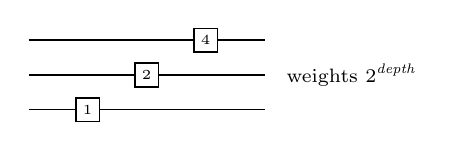
\begin{tikzpicture}[x=5mm,y=4.4mm,line width=0.6pt]
  \foreach \y in {0,1,2} \draw (0,\y) -- (6,\y);
  \node[draw,fill=white,font=\tiny,minimum size=3mm,inner sep=0pt] at (1.5,0) {$1$};
  \node[draw,fill=white,font=\tiny,minimum size=3mm,inner sep=0pt] at (3,1) {$2$};
  \node[draw,fill=white,font=\tiny,minimum size=3mm,inner sep=0pt] at (4.5,2) {$4$};
  \node[font=\scriptsize,anchor=west] at (6.3,1) {weights $2^{\mathit{depth}}$};
\end{tikzpicture}

\vspace{2pt}
{\scriptsize Scope today: the \emph{structural} rules. No gate-specific rule set is
shown minimal yet --- but several were \emph{reduced} by derivations
(next slides).}
\end{column}
\end{columns}
\end{frame}
